\chapter{Introduction}
\label{chap:intro}

\makeatletter
\newenvironment{chapquote}[2][2em]
{\setlength{\@tempdima}{#1} \def\chapquote@author{#2} \parshape 1
  \@tempdima \dimexpr\textwidth-2\@tempdima\relax \itshape}
{\par\normalfont\hfill--\
\chapquote@author\hspace*{\@tempdima}\par\bigskip}
\makeatother

\begin{chapquote}{Alan Turing}
  ``I propose to consider the question: Can machine think?''
\end{chapquote}
The ultimate goal of image understanding is to transfer the visual
signals (images/videos) into abstract symbolic descriptions of the
world which are helpful for decision making.
However, understanding images is a not trivial task for machines.
In order to handle various complicated scenarios, researchers divide
image understanding into different computer vision tasks: Pedestrian
detection for autonomous driving, and image retrieval for image
searching engines \etc.

For many applications, knowing when, where, and in which direction a
picture was taken is important to understand the world. We refer to 
estimating these properties as the task of  {\em geo-calibration}.
In current work of geo-calibration, most algorithms are
deterministic, which means they output fixed solutions. Deterministic
systems may seem straight-forward but they also have some obvious
drawbacks: 1) Deterministic systems can not model the inherent
uncertainties from images of ambiguous scenes. 2) They are not
friendly to applications that take probabilistic inputs. To address
these problems, We propose to build probabilistic models for camera
geo-calibration.

Feature engineering is essential for image understanding. In recent
years, learning based approaches for high-level feature construction
like deep neural nets get popular. However, most of these feature
learning methods heavily relies on manually labeled data. In our
thesis, we presented alternative ways to learn high-level image
representations when the manually labeled data is either insufficient
or absent. We show that learning to geo-calibrate a camera is helpful
for high-level feature extracting.

\begin{figure}
  \centering
  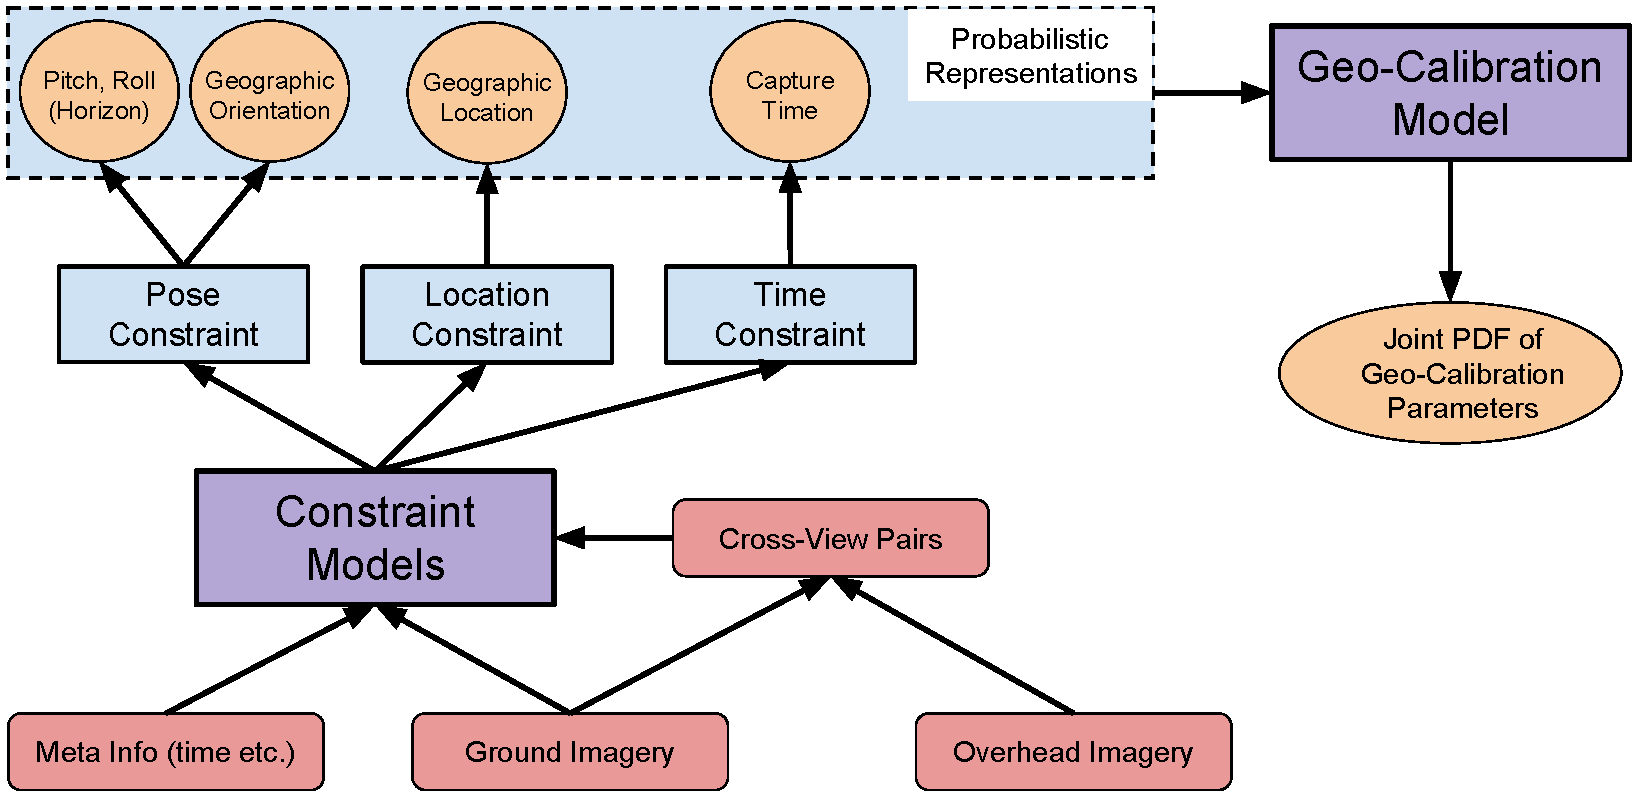
\includegraphics[width=.8\linewidth]{introduction/architecture}
  \caption{Architecture of our approach.}
  \label{fig:intro:architecture}
\end{figure}

\section{Background}

\subsection{Geo-Calibration}
\todo{add deterministic methods, add literature for time estimation}

Automatic image geo-calibration continues to grow in importance as a
direct result of the increasing amount of imagery available
via the Internet. Conceptually geo-calibration task is
straightforward: given an image, identify the time and the location it
was captured in the world and the direction the camera was facing.
Solving this problem is of great value for a wide variety of fields,
with potential applications ranging from the forensic
sciences~\cite{stylianou13jane} to crowd-sourced environmental
monitoring~\cite{zhang2012mining}.

Extracting location-dependent or orientation-dependent features from
image data has drawn a great detail of attention from the vision
community~\cite{jacobs07geolocate, jacobs11geolocate,
jacobs08geoorient}. The common trend amongst these methods is that
they take advantage of a large dataset of geo-referenced images. Hays
and Efros~\cite{hays2008im2gps} use a data-driven scene matching
approach to localize a query image using a large dataset of geo-tagged
images.  Doersch et al. extract location-dependent features that
capture the relative appearance differences of large cities.  Lin et
al.~\cite{lin2013cross} localize a ground-level image by learning the
relationship between pairs of ground and aerial images of the same
location. Other techniques focus on urban environments and infer
location using local image
descriptors~\cite{schindler2008detecting,snavely2006photo}. Li et
al.~\cite{li2012worldwide} exploit geo-registered 3D points clouds to
estimate camera pose. Many other cues exist, such as the
skyline~\cite{baatz2012large,ramalingam2009geolocalization}, sky
appearance~\cite{lalonde2010sun,workman2014rainbow}, and
shadows~\cite{junejo2008estimating,wu2010geo}.

However, recognizing the geo-location and geo-orientation of an
arbitrary outdoor image is an extremely challenging task.  Many
methods have been proposed; the most common approach is to build a
large database of images with known location and localize a query
image using either local~\cite{li2010location,schindler2008detecting}
or global~\cite{hays2008im2gps,doersch2012what} image features.  This
approach is not applicable when no nearby ground-level imagery exists
in the reference database, such as when the image was not captured
near a popular tourist destination.  Even when reference imagery is
available, the appearance of the objects may not be visually
distinctive, for example a train track or a body of water. 


\subsection{Deep Neural Networks for Geo-Calibration}
In recent years, deep neural networks (DNNs) were proven to be
extremely successful in many computer vision areas (\todo{citations}). 
The deep neural networks prove to be a good tool to extract high-level
image representations, this valuable ability offers great help for researchers
to conquer the problems like geo-localization and camera calibration.
Recent work on cross-view image
geo-localization~\cite{lin2013cross,lin2015learning,workman2015geocnn,workman2015wide}
has shown that convolutional neural networks are capable of extracting
features from geo-tagged aerial imagery that can be matched to features extracted
from the inquiry ground imagery.  Vo \etal~\cite{vo2016localizing} extend this
line of work, demonstrating improved geo-localization performance by
applying an auxiliary loss function to regress the ground-level camera
orientation with respect to the aerial image. 

Closely related to camera geo-calibration, studies also have been done
to identify the camera poses and focal length using deep neural
networks.
Horizon line is an important indicator for estimating camera poses,
which is, giving the focal length, one can derive the camera roll and
pitch angles from the horizon line position in the image.
Work~\cite{zhai2016horizon, workman2016horizon, hold2017perceptual}
has been done to to identify the horizon line with CNNs.  Workman
\etal~\cite{workman2015deepfocal} develop a CNN to estimate the camera
focal length. Kendall \etal~\cite{kendall2015convolutional} propose a
neural network that can identify 6-DOF camera parameters, but their
method only limited to specific scenes.

\subsection{Ground-to-Aerial Geo-Calibration}
Data-driven scene matching approaches are widely used to localize a
query image by registering in a large dataset of geo-tagged images. 
Benefited from the fast growing monitoring satellite market, overhead
imagery grows fast nowadays, which also makes it a perfect source for
database of geo-tagged. We refer to the geo-calibration process of
matching the ground-level imagery to the aerial imagery as {\em
Ground-to-Aerial Geo-Calibration}.
%
Cross-view image pair is the basic element for ground-to-aerial
geo-calibration. It consists of a ground-level image and an overhead
image at the same location. In some cases, two images are also aligned
in orientation. 

\todo{cite ground-to-aerial geo-calibration papers}

\section{\todo{Dataset}}
Introduce the dataset we use.

\section{Our Approach}
Our approach consists of two big steps. First, we propose a general
probabilistic model to jointly estimate the geo-calibration
parameters. The key for the success of this model is to construct good
constraint functions which describe the fitness between the calibration
parameters and the images. As the second step of our approach, we
dismantle the full geo-calibration into several partial
geo-calibration tasks, each of which could provides a strong constraint
function that fit in the general model. The architecture of
our approaches refers to \figref{intro:architecture}.
%
In the end, we show that learning to geo-calibrate a camera is helpful
for high-level image feature extracting.


\subsection{General Probabilistic Model for Geo-Calibration}
The complete camera geo-calibration detects the camera
geographic location, pose, and focal length of the camera.  We
design a general model to estimate the probability over these
geo-calibration parameters: First, we model the relationship between the
image projection of the scene and the geo-calibration parameters. This
relationship can be described by the pin-hole model, and
the geographic location of the camera.
We then construct a scoring function to measure the ``fitness'' between the
calibration parameters and the observation of the image. 
The scoring function is proportional to the probability distribution
of the camera parameters. We propose a Markov Chain Monte
Carlo (MCMC) sampling approach to approximate the underlying
probability distribution over the full geo-calibration of the camera.
Our model is a general architecture, which can take different
constraints to form the scoring function. The details about this model
can be found in \chapref{mcmc}.

\subsection{Developing Constraint Functions}
In our general model, the scoring function is defined as a linear
combination of multiple constraint functions.
In the rest of the work, we focus on developing good constraint
functions for different set of calibration parameters. 

\begin{itemize}[noitemsep]
  \item \textbf{Constraint for Horizon Line and Vanishing Points:}
  We first estimate camera roll and pitch angles. Assuming the intrinsic
  parameters are known, camera roll and pitch angles can be
  derived from the horizon line position in the image. Compared to
  directly detecting the camera pose, identifying horizon line is easier
  because it is tightly related to the appearance
  of the scene. In our work, we create a new method using CNN to
  estimate the prior distribution of the horizon line. We assign
  a probability to each horizon line by measuring their consistences
  with vanishing points detected using traditional statistic methods.
  We present the algorithm details in \chapref{fasthorizon}.
  \newline

  \item \textbf{Constraint for Coarse Geographic Locations:}
  In this work, we demonstrate to estimate the camera geographic
  location with the input image.
  We provide two approaches to obtain the probability distribution over the camera
  geographic location. Most straightforwardly, our network estimate the
  categorical distribution over world into a $N \times M$ bins. Better
  results can be procured with temporal inputs (image timestamps).
  Our algorithm can also compute the probability at arbitrary
  geographic location, with lower accuracy than the straightforward
  method.
  We demonstrate that our algorithm is able to learn geo-temporal
  image representations with geographic locations and capture
  time.
  We present the algorithm details in \chapref{whenwhere}.
  \newline

  \item \textbf{Constraint for Fine Geographic Locations and Orientations}
  In our previous method, we present that our algorithm can estimate
  the camera location distribution in low-res world division. In this
  work we focus on refining the geo-localization results with the help
  of overhead imagery and on estimating the camera geo-orientation.
  Current machine learning methods address problems that involves mostly
  the ground imagery. Tons of dataset targeting on ground imagery are
  annotated while much fewer are done for the overhead imagery.
  In this work, we try to transfer the semantics from the ground imagery
  to the overhead imagery by identifying the latent geometry
  correspondences between these two. Similar to the monocular depth
  estimation methods that driven by
  the technique called {\em Reprojection
  Losses}~\cite{garg2016unsupervised,
  godard2017unsupervised,zhou2017unsupervised, yan2016perspective}, our
  network learns to geometrically project pixels from the overhead
  images to the ground images,
  and learns to segment the overhead images jointly. 
  When refining the camera geographic location, we compare the
  semantic layout of the ground image with those transferred from
  overhead images sampled from different locations and orientations. The
  optimal prediction is found when the semantic layouts from these
  two sources match best. For probabilistic outputs, we assign
  a score to each location and orientation setting,
  based on how well the semantic layouts match to each other.
  We present the algorithm details in \chapref{crosstransf}
  \newline

\end{itemize}


\section{Geo-Calibration for Feature Learning}

Automatic feature engineering has drawn a lot of attention over the
past years in the computer vision community due to its efficiency and
not requiring expert knowledge about the data.  In recent years, deep
neural networks are acknowledged as good tools to learn high-level
features for image understanding.  As parametric algorithms, deep
neural networks require training for their parameters.  Methods to
train deep neural networks include supervised algorithms, unsupervised
algorithms, and reinforcement learning. Supervised algorithms are the
most popular and commonly applied in many computer vision areas,
thanks to their good performances and the fact that they are easy to
implement. However, supervised learning approaches are sensitive to
the quality of data annotations. In some applications like overhead
image segmentation and transient attributes estimation, data with
noise-free annotation is either very limited in quantity or
technically difficult to acquire.  In this thesis, Our methods focus
on lavaging the camera geographic information to deal with the
challenges of lacking noise-free annotations during DNN training. The
insight is that the camera geographic information encodes the semantic
information because it is related to the appearances of the scenes.
